% SutureAI visual design spec — current stage (warm paper).
% Build (from docs/design, with the app running for the figures):
%   python tools/prepare-fonts.py                     # Barlow TTFs from node_modules
%   node tools/capture-figures.mjs http://localhost:5173
%   latexmk -xelatex -outdir=build sutureai-design-spec.tex
\documentclass[10pt,a4paper]{article}

\usepackage[margin=2.1cm,top=2.3cm,bottom=2.3cm]{geometry}
\usepackage{fontspec}
\usepackage{xcolor}
\usepackage{graphicx}
\usepackage{tikz}
\usepackage{booktabs,tabularx,array,longtable}
\usepackage{enumitem}
\usepackage[most]{tcolorbox}
\usepackage{titlesec}
\usepackage{fancyhdr}
\usepackage{caption}
\usepackage[hidelinks]{hyperref}
\usepackage{float}
\usepackage{needspace}

\newcolumntype{L}[1]{>{\raggedright\arraybackslash}p{#1}}
\newcolumntype{Y}{>{\raggedright\arraybackslash}X}

% ---- fonts (the app's own pair) --------------------------------------------------
\setmainfont{Montserrat-Regular.otf}[
  BoldFont=Montserrat-SemiBold.otf,
  ItalicFont=Montserrat-Italic.otf,
  BoldItalicFont=Montserrat-SemiBoldItalic.otf]
\setmonofont{SourceCodePro-Regular.otf}[Scale=0.92]
\newfontfamily\display{Barlow-SemiBold.ttf}[Path=build/fonts/, BoldFont=Barlow-Bold.ttf]
\newfontfamily\cjk{Microsoft YaHei}

% ---- palette (matches tailwind.config.js) ------------------------------------------
\definecolor{paper}{HTML}{F8F6F1}
\definecolor{tile}{HTML}{F2EFE9}
\definecolor{line}{HTML}{E8E3D8}
\definecolor{mist}{HTML}{D9D3C6}
\definecolor{ink}{HTML}{2B2924}
\definecolor{inksoft}{HTML}{4A463F}
\definecolor{muted}{HTML}{6F6A60}
\definecolor{brand}{HTML}{4F69C2}
\definecolor{brandfifty}{HTML}{F1F4FC}
\definecolor{brandtwo}{HTML}{C5D1F0}
\definecolor{brandthree}{HTML}{9DB0E3}
\definecolor{brandeight}{HTML}{26365F}
\definecolor{good}{HTML}{4A7456}
\definecolor{warn}{HTML}{8C6A22}
\definecolor{bad}{HTML}{A24E36}

\pagecolor{paper}
\color{ink}
\hypersetup{colorlinks=true,linkcolor=brand,urlcolor=brand}
\setlength{\parindent}{0pt}
\setlength{\parskip}{0.55em}
\linespread{1.12}
\setlist{itemsep=0.15em,topsep=0.3em}
\graphicspath{{build/figures/}}

% Section labels follow the app: blue number, Barlow title.
\titleformat{\section}{\display\LARGE\bfseries\color{brandeight}}{\color{brand}\normalsize\thesection\hspace{0.35em}}{0.4em}{}
\titleformat{\subsection}{\display\Large\color{brandeight}}{\color{brand}\small\thesubsection}{0.6em}{}
\titlespacing*{\section}{0pt}{1.8em}{0.6em}
\titlespacing*{\subsection}{0pt}{1.2em}{0.35em}
\makeatletter\renewcommand{\thesection}{\two@digits{\value{section}}}\makeatother

\captionsetup{font={small,color=muted},labelfont={bf,color=muted},skip=6pt}

\pagestyle{fancy}
\fancyhf{}
\renewcommand{\headrulewidth}{0pt}
\fancyhead[L]{\small\color{muted}SutureAI · Visual Design Spec}
\fancyhead[R]{\small\color{muted}\leftmark}
\fancyfoot[C]{\small\color{muted}\thepage}
\renewcommand{\sectionmark}[1]{\markboth{#1}{}}

% ---- helpers ------------------------------------------------------------------------
\newcommand{\code}[1]{\leavevmode{\ttfamily\small\color{brandeight}#1}}
\newcommand{\hex}[1]{\leavevmode{\ttfamily\small #1}}

% Swatch: \swatch{HEX}{name}{role}
\newcommand{\swatch}[3]{%
  \begin{tikzpicture}[baseline=-0.6ex]
    \definecolor{sw}{HTML}{#1}
    \fill[sw, draw=black!12, rounded corners=1.5pt] (0,-0.22) rectangle (0.9,0.22);
  \end{tikzpicture}\hspace{0.5em}\textbf{#2}\hfill\hex{\##1}\par
  {\small\color{muted}#3}\par\smallskip}

% Grey tile, dashed tile and blue tile, as in the app.
\newtcolorbox{tilebox}[1][]{enhanced, colback=tile, colframe=tile, boxrule=0pt, arc=4pt,
  left=10pt,right=10pt,top=8pt,bottom=8pt, #1}
\newtcolorbox{dashedbox}[1][]{enhanced, colback=tile, frame hidden, arc=4pt,
  borderline={0.8pt}{0pt}{brandthree,dashed}, left=10pt,right=10pt,top=8pt,bottom=8pt, #1}
\newtcolorbox{bluebox}[1][]{enhanced, colback=brandfifty, colframe=brandfifty, boxrule=0pt, arc=4pt,
  left=10pt,right=10pt,top=8pt,bottom=8pt, #1}

\newcommand{\tiletitle}[2][brand]{{\display\large\color{brandeight}\textcolor{#1}{\raisebox{0.15ex}{\tikz\fill (0,0) circle (2.4pt);}}\hspace{0.45em}#2}\par\smallskip}

% Open question block: number, question, recommendation.
\newcounter{oq}
\newenvironment{question}[1]{%
  \stepcounter{oq}%
  \begin{tilebox}[before skip=6pt, after skip=6pt]
  {\display\large\color{brandeight}\textcolor{brand}{Q\theoq}\hspace{0.5em}#1}\par\smallskip}
  {\end{tilebox}}
\newcommand{\recommend}[1]{\par\smallskip{\small\textbf{\color{brand}Recommendation.}\ #1}}

\begin{document}

% ================================================================================
% Title
% ================================================================================
\thispagestyle{empty}
\begin{tikzpicture}[remember picture, overlay]
  \fill[brand] (current page.north west) rectangle ([yshift=-0.35cm]current page.north east);
\end{tikzpicture}

\vspace*{2.2cm}
{\small\color{muted}\MakeUppercase{SutureAI} \textperiodcentered\ Design \textperiodcentered\ Stage 2}\par
\vspace{0.4cm}
{\display\fontsize{40}{44}\selectfont\bfseries\color{brandeight}Visual Design Spec}\par
\vspace{0.2cm}
{\Large\color{inksoft}Warm paper, blue and white}\par
\vspace{0.9cm}

% Stitched incision, the product's ornament.
\begin{tikzpicture}[x=0.05cm,y=-0.05cm]
  \draw[brandtwo, line width=1.1pt, line cap=round] (10,70) .. controls (70,30) and (130,95) .. (190,55) .. controls (250,15) and (300,30) .. (350,60);
  \foreach \a/\b/\c/\d [count=\i, evaluate=\i as \op using 0.45+0.06*\i] in {38/42/50/70, 76/46/84/72, 114/56/120/82, 152/58/156/84, 190/44/192/70, 228/34/232/60, 266/30/272/56, 304/38/312/62}
    \draw[brand, line width=1.1pt, line cap=round, opacity=\op] (\a,\b) -- (\c,\d);
\end{tikzpicture}

\vspace{1.2cm}
\begin{tabularx}{\textwidth}{@{}>{\leavevmode\color{muted}}L{3.2cm}Y@{}}
Status & Draft for alignment \\
Date & 18 October 2026 \\
Branch & \code{feat/ui-polish} (report-page sample committed as \code{5655735}; later rounds not yet committed) \\
Scope & Every screen of the web app: login, student dashboard, training \& processing, report, instructor overview, student detail, review queue. The print/PDF export view is not restyled yet (see Q5). \\
Source of truth & \code{tailwind.config.js} (tokens) and \code{src/index.css} (component classes). This document describes them; where they disagree, the code wins.
\end{tabularx}

\vfill
\begin{bluebox}
\textbf{What this document is for.} It records the visual direction we have converged on, the
rules that keep the screens consistent, and the decisions that are still open. Section~\ref{sec:open}
lists the questions to settle before the remaining polish and the PR.
\end{bluebox}

\newpage
\tableofcontents
\newpage

% ================================================================================
\section{Summary}
% ================================================================================

The interface moves from a cool, generic dashboard look to a \textbf{warm paper} look taken from
the ENT111 roadshow deck: white sheets on a warm off-white ground with a fine grain, one calm blue
as the main colour, warm greys for text, and status colours that are muted but still pass contrast.
Decoration is replaced by editorial typography (numbered sections, small-caps labels, dotted leader
rows) and motion is \emph{drawn} (pen strokes, count-ups) rather than floating.

\subsection{How we got here}

\begin{tabularx}{\textwidth}{@{}L{2.6cm}Y@{}}
\toprule
\textbf{Round} & \textbf{Outcome} \\
\midrule
v1 Glass & Periwinkle gradients, frosted cards, glossy 3D icon badges, floating colour blobs. Rejected: the 3D icons did not look good and the overall feel was too ornamental. Kept as a patch backup only. \\
Exploration & Two paper variants side by side (\code{docs/design/paper-style-tiles.html}): A warm paper + ink blue, B cool paper + slate blue. \\
v2 Warm paper & Chosen: warm paper \emph{with blue and white kept as the main tones}. Barlow for titles (serif titles considered and not taken). Sampled on the report page, then rolled out to every page. \\
v2.1 Tiles & Added borderless grey tiles and dashed grey tiles (from the deck's pricing slide); re-laid out the dashboard welcome card. \\
\bottomrule
\end{tabularx}

\subsection{Decisions already made}

\begin{itemize}
  \item Fonts: \textbf{Barlow} (titles, numbers) + \textbf{Montserrat} (body), bundled with \code{@fontsource}, no CDN. Chinese: system fonts for now.
  \item Motion library: \textbf{Motion} (\code{motion/react}); icons: \textbf{lucide-react} plus hand-drawn suturing icons.
  \item Warm paper ground, white sheets, blue as the single main colour; no glass, no gradients on surfaces.
  \item Grey borderless tiles and dashed grey tiles as the standard way to group content inside a sheet.
\end{itemize}

% ================================================================================
\section{Principles}
% ================================================================================

\begin{enumerate}[leftmargin=1.4em, itemsep=0.5em]
  \item \textbf{Paper, not glass.} Surfaces are flat: white sheets with a hairline edge and an almost
        invisible shadow on a warm ground. No blur, no translucent layers, no gradient fills.
  \item \textbf{One main colour.} Blue marks what is interactive or important. Everything else is warm grey.
  \item \textbf{Colour carries meaning, never decoration.} Green / ochre / brick appear only for good /
        warning / problem, and always next to an icon or a word.
  \item \textbf{Typography carries hierarchy.} Numbered sections, small-caps labels with a hairline rule,
        Barlow for titles and figures. Boxes are the last resort.
  \item \textbf{Draw, don't float.} Animations look like a pen drawing on paper: strokes, counts and
        fills. Nothing bounces or hovers upward. All motion respects \emph{reduce motion}.
\end{enumerate}

% ================================================================================
\section{Colour}
% ================================================================================

\subsection{Surfaces and ink}

\noindent
\begin{minipage}[t]{0.47\textwidth}
\swatch{F8F6F1}{paper}{Page ground, with an SVG grain at 55\,\% multiply.}
\swatch{FFFFFF}{sheet}{Cards (\code{surface-card}).}
\swatch{F2EFE9}{tile}{Borderless grey tile inside a sheet.}
\swatch{E8E3D8}{line}{Hairlines, card edges, dividers.}
\swatch{D9D3C6}{mist}{Inputs, dotted leaders, inactive marks.}
\end{minipage}\hfill
\begin{minipage}[t]{0.47\textwidth}
\swatch{2B2924}{ink}{Body text, values.}
\swatch{4A463F}{ink-soft}{Secondary text, list items.}
\swatch{6F6A60}{ink-muted}{Labels, captions, hints.}
\swatch{26365F}{brand-800}{Titles.}
\swatch{4F69C2}{brand-500}{Main blue: buttons, active state, numbers.}
\end{minipage}

\subsection{Brand ramp}

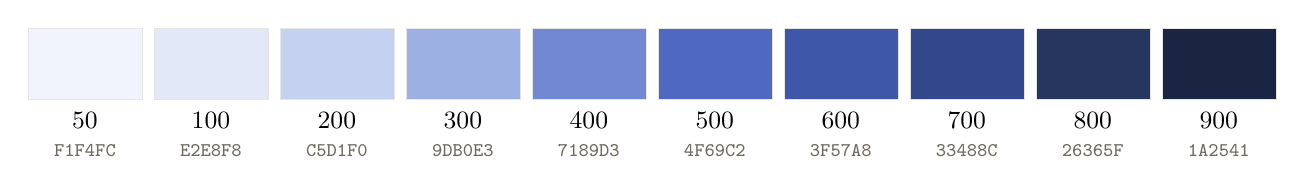
\begin{tikzpicture}
  \foreach \h/\n [count=\i from 0] in {F1F4FC/50, E2E8F8/100, C5D1F0/200, 9DB0E3/300, 7189D3/400, 4F69C2/500, 3F57A8/600, 33488C/700, 26365F/800, 1A2541/900} {
    \definecolor{c}{HTML}{\h}
    \fill[c, draw=black!10] (\i*1.6,0) rectangle ++(1.45,0.9);
    \node[anchor=north, font=\small] at (\i*1.6+0.72,-0.05) {\n};
    \node[anchor=north, font=\ttfamily\scriptsize, text=muted] at (\i*1.6+0.72,-0.45) {\h};
  }
\end{tikzpicture}

The heatmaps (training calendar, instructor skill map) use the same blues: a 13-step ramp
interpolated from brand-100 to brand-800, with white numbers from step 6 up.

\subsection{Status}

\noindent
\begin{minipage}[t]{0.31\textwidth}
\swatch{4A7456}{good}{Completed, met target, upward change.}
\end{minipage}\hfill
\begin{minipage}[t]{0.31\textwidth}
\swatch{8C6A22}{warn}{Warnings, pending review, confidence notices.}
\end{minipage}\hfill
\begin{minipage}[t]{0.31\textwidth}
\swatch{A24E36}{bad}{Problems, points lost, failures.}
\end{minipage}

The Tailwind \code{slate}, \code{emerald}, \code{amber} and \code{rose} scales are
\textbf{remapped} onto this palette in \code{tailwind.config.js}, so existing classes across the app
follow it without code changes (trade-off discussed in Q1). \code{indigo} was replaced by \code{brand}.

\subsection{Contrast}

Every text colour reaches WCAG AA (4.5:1) on the surfaces it is used on. Values below are measured;
the one shortfall found while writing this document (warn on a grey tile) has been fixed by using
\code{amber-700} there.

\smallskip
\begin{tabularx}{\textwidth}{@{}Xrrrr@{}}
\toprule
\textbf{Text colour} & \textbf{on white} & \textbf{on paper} & \textbf{on grey tile} & \textbf{on blue tile} \\
\midrule
ink \hex{\#2B2924}       & 14.5 & 13.5 & 12.7 & 13.2 \\
ink-soft \hex{\#4A463F}  & 9.4  & 8.7  & 8.2  & 8.5 \\
ink-muted \hex{\#6F6A60} & 5.4  & 5.0  & 4.7  & 4.9 \\
brand-800 \hex{\#26365F} & 11.8 & 11.0 & 10.3 & 10.8 \\
brand-600 \hex{\#3F57A8} & 6.7  & 6.2  & 5.8  & 6.1 \\
brand-500 \hex{\#4F69C2} & 5.1  & 4.7  & \textcolor{warn}{4.4}$^{*}$ & 4.6 \\
good \hex{\#4A7456}      & 5.4  & 5.0  & 4.7  & 4.9 \\
warn \hex{\#8C6A22}      & 5.0  & 4.6  & \textcolor{warn}{4.4}$^{*}$ & 4.5 \\
bad \hex{\#A24E36}       & 5.7  & 5.3  & 5.0  & 5.2 \\
\bottomrule
\end{tabularx}

{\small\color{muted}$^{*}$ Not used as body text on grey tiles. Rule: on a grey tile, use brand-600+ and amber-700 for text.}

% ================================================================================
\section{Typography}
% ================================================================================

\begin{tabularx}{\textwidth}{@{}L{3.3cm}L{4.4cm}Y@{}}
\toprule
\textbf{Role} & \textbf{Face} & \textbf{Where} \\
\midrule
{\display\Large\bfseries\color{brandeight}Page title} & Barlow Bold 30--36\,px & \code{title-display}: one per page. \\
{\display\large\color{brandeight}Section title} & Barlow SemiBold 20\,px & \code{section-title}, led by a blue two-digit number. \\
{\scriptsize\color{muted}\MakeUppercase{Section label}} & Montserrat 11\,px caps, 0.16em & \code{pill-header}: small caps label with a hairline to the right. \\
{\display\Large\bfseries\color{brand}66} & Barlow Bold 30--60\,px & Scores and KPIs, tabular figures. \\
Body & Montserrat 14\,px & Paragraphs, list items, table cells. \\
{\ttfamily\small 0:26} & System mono 12\,px & Timestamps and file details. \\
\bottomrule
\end{tabularx}

Barlow and Montserrat have no Chinese glyphs; Chinese text falls back to the system UI font
(Microsoft YaHei / PingFang). Mixed-language titles therefore change face mid-line (Q4).

% ================================================================================
\section{Surfaces and components}
% ================================================================================

\Needspace{18\baselineskip}
\subsection{Containers}

Four containers, from loudest to quietest. A sheet sits on the paper; tiles sit inside a sheet.
Tiles never nest.

\smallskip
\noindent
\begin{minipage}[t]{0.48\textwidth}
\begin{tcolorbox}[enhanced, colback=white, colframe=line, boxrule=0.5pt, arc=4pt, left=10pt, right=10pt]
\textbf{Sheet} \code{surface-card}\par
{\small\color{muted}White, hairline edge, faint shadow. Page sections. May carry a 4\,px blue top rule when it is the page's hero.}
\end{tcolorbox}
\end{minipage}\hfill
\begin{minipage}[t]{0.48\textwidth}
\begin{bluebox}
\tiletitle{Blue tile \code{tile-blue}}
{\small\color{muted}No border, light blue fill. At most one per card: the thing to read first (AI feedback, next practice priorities).}
\end{bluebox}
\end{minipage}

\smallskip
\noindent
\begin{minipage}[t]{0.48\textwidth}
\begin{tilebox}
\tiletitle[good]{Grey tile \code{tile}}
{\small\color{muted}No border, warm grey fill. Groups related content: strengths, improvements, notices, demo accounts.}
\end{tilebox}
\end{minipage}\hfill
\begin{minipage}[t]{0.48\textwidth}
\begin{dashedbox}
\tiletitle{Dashed tile \code{tile-dashed}}
{\small\color{muted}Dashed blue outline on grey. Optional, private or ``ready to start'' content: next steps, personal note, evidence clips, the dashboard start tile.}
\end{dashedbox}
\end{minipage}

Tile titles (\code{tile-title}) lead with a small dot. The dot takes the tone: blue by default,
\code{is-good}, \code{is-bad}, \code{is-warn} for status.

\subsection{Editorial pieces}

\begin{tabularx}{\textwidth}{@{}L{3.6cm}Y@{}}
\toprule
\textbf{Class} & \textbf{Use} \\
\midrule
\code{section-title} + \code{section-num} & Numbered section heading (01, 02, \dots) on every page except the instructor views, which use unnumbered titles. \\
\code{pill-header} & Small-caps label with a hairline; names a card or tile. \\
\code{leader} & ``Label \textperiodcentered\textperiodcentered\textperiodcentered\ value'' rows. Replaces bordered key/value boxes. Label stays on one line; long values wrap right-aligned (see Q7). \\
\code{stamp} & Rotated rubber stamp for the report's review status; drops in with a short ``stamp'' animation. \\
\code{chip} & Outlined, square-cornered tag for types and states (problem, warning, metrics). \\
\bottomrule
\end{tabularx}

\subsection{Controls}

\begin{tabularx}{\textwidth}{@{}L{3.6cm}Y@{}}
\toprule
\code{btn-primary} & Solid brand-500, white text, darkens on hover. One per area. \\
\code{btn-secondary} & White with a mist border; text and border turn blue on hover. \\
\code{btn-ghost} & Blue text link with an underline on hover; inline actions (Replay, View, Log out). \\
\code{field-input}, \code{field-select} & White, mist border, blue focus ring. \\
Segmented control & Language switch and the report's view-mode switch; the active pill slides (Motion \code{layoutId}). \\
\bottomrule
\end{tabularx}

% ================================================================================
\section{Iconography}
% ================================================================================

\begin{itemize}
  \item \textbf{lucide-react} line icons for everything generic, at 1.5--1.75 stroke, in brand or ink colours.
        No fills, no gradients, no 3D.
  \item \textbf{Hand-drawn suturing icons} (\code{src/components/icons/DomainIcons.jsx}) on the same
        24\,px grid and stroke props: Needle, Stitch, NeedleHolder, Knot, ARGlasses, HandTrack.
        Used where lucide has nothing (e.g. Product Quality, empty states).
  \item \code{IconBadge}: a line icon in a hairline circle (white or tinted). Replaces the glossy badges of v1.
  \item The \textbf{stitched incision} (\code{SutureLine}) is the product's ornament: login brand panel,
        report hero, dashboard welcome. It is drawn, never filled.
\end{itemize}

% ================================================================================
\section{Motion}
% ================================================================================

Built on Motion (\code{motion/react}) with a few shared primitives in
\code{src/components/motion}. \code{MotionConfig reducedMotion="user"} switches transforms off for
users who ask for less motion; \code{CountUp} checks the setting itself.

\smallskip
\begin{tabularx}{\textwidth}{@{}L{3.6cm}YL{2.6cm}@{}}
\toprule
\textbf{Element} & \textbf{Motion} & \textbf{Timing} \\
\midrule
Sections (\code{Reveal}) & Fade in, 6--8\,px rise, once, when scrolled into view & 0.5--0.6\,s ease-out \\
Card groups (\code{Stagger}) & Children fade in one after another & 70\,ms apart \\
Score ring & Arc drawn from 0 to the score, number counts up with it & 1.4\,s \\
Bars (\code{GrowBar}) & Fill grows from the left; staggered per row & 1.0\,s \\
Radar & Polygon grows from the centre, then the points appear & 1.0\,s \\
Stitched incision & Cut drawn first, then each stitch crosses it & 1.4\,s + 0.1\,s / stitch \\
Processing bar & Progress drawn as a suture: a stitch pops in at every 5\,\% & per poll \\
Timeline & Expand / collapse animates height; filtering animates layout & 0.35\,s \\
Status stamp & Drops in from 1.5$\times$ scale & 0.5\,s, 0.6\,s delay \\
Hover & Colour and border only. No lift, no shadow growth & 0.2--0.3\,s \\
\bottomrule
\end{tabularx}

% ================================================================================
\section{Screens}
% ================================================================================

All figures: 1280\,px wide, English UI, demo data, captured by \code{tools/capture-figures.mjs}.

\begin{figure}[H]
  \centering\includegraphics[width=\textwidth]{login}
  \caption{Login. Brand panel with the stitched incision and three numbered promises; the form sheet with a dashed hint tile and a grey demo-accounts tile.}
\end{figure}

\begin{figure}[H]
  \centering\includegraphics[width=\textwidth]{dashboard}
  \caption{Student dashboard. Account controls moved into a top bar; the welcome sheet pairs the greeting with a dashed ``current training task'' tile holding both calls to action. Numbered sections below use leader rows.}
\end{figure}

\begin{figure}[H]
  \centering\includegraphics[width=\textwidth]{report-top}
  \caption{Report, top. Hero sheet with blue top rule, review stamp and incision ornament; meta row with line icons; overall score drawn as an arc, with leader rows and a grey confidence tile.}
\end{figure}

\begin{figure}[H]
  \centering\includegraphics[width=\textwidth]{report-dimensions}
  \caption{Report, dimension scores. Radar grows from the centre; each dimension card counts up and fills its bar.}
\end{figure}

\begin{figure}[H]
  \centering\includegraphics[width=\textwidth]{report-timeline}
  \caption{Report, timeline and highlights. Small status dots on a hairline spine; text actions (Replay, Collapse, Appeal) instead of boxed buttons.}
\end{figure}

\begin{figure}[H]
  \centering\includegraphics[width=\textwidth]{report-feedback}
  \caption{Report, feedback. Blue tile for AI feedback; grey tiles for strengths and improvements (dot shows the tone); dashed tiles for next steps and the private note.}
\end{figure}

\begin{figure}[H]
  \centering\includegraphics[width=\textwidth]{processing}
  \caption{Processing. Large Barlow percentage, suture-style progress bar, stage checklist, and the activity log on deep navy.}
\end{figure}

\begin{figure}[H]
  \centering\includegraphics[width=\textwidth]{instructor}
  \caption{Instructor overview. Ledger-style tab bar, Barlow KPI tiles, outlined severity chips, skill map on the brand ramp.}
\end{figure}

% ================================================================================
\section{Implementation notes}
% ================================================================================

{\small
\begin{tabularx}{\textwidth}{@{}L{6.4cm}Y@{}}
\toprule
\textbf{File} & \textbf{Holds} \\
\midrule
\code{tailwind.config.js} & Palette (brand, ink, paper, line, mist, status), remapped slate/emerald/amber/rose, fonts, shadows, keyframes. \\
\code{src/index.css} & Paper grain, sheets, tiles, labels, stamp, leaders, buttons, fields, skeleton. \\
\code{src/components/motion/} & Reveal, Stagger, CountUp, GrowBar, shared easing. \\
\code{src/components/icons/} & DomainIcons, IconBadge. \\
\code{src/components/decor/SutureLine.jsx} & The stitched incision. \\
\code{src/components/charts/tokens.js} & Chart colours and the heatmap ramp, aligned with the palette. \\
\code{docs/design/} & This spec, its figure and font tools, and the paper-style comparison page. \\
\bottomrule
\end{tabularx}
}

\textbf{Known caveats.}
\begin{itemize}
  \item Production bundle is 525\,kB (164\,kB gzip), above Vite's 500\,kB warning (Q6).
  \item Content that enters with an animation is invisible until the animation runs. In a background
        tab the browser pauses animation frames, so screenshots from hidden tabs can look empty; real
        foreground use is unaffected.
\end{itemize}

% ================================================================================
\section{Open questions}\label{sec:open}
% ================================================================================

Each question has a recommendation so we can move fast; anything you agree with I will implement as written.

\begin{question}{Remap Tailwind scales, or rename the classes?}
The warm palette reaches older screens because \code{slate}, \code{emerald}, \code{amber} and
\code{rose} are redefined. It works today, but the names now lie (``emerald'' is a muted sage) and a
new contributor reaching for \code{rose-500} will not get Tailwind's rose.
\recommend{Keep the remap for this PR; in a follow-up, rename usages to semantic tokens (\code{ink-*}, \code{good}, \code{warn}, \code{bad}) and drop the overrides.}
\end{question}

\begin{question}{The dashboard shows the current task twice}
The welcome sheet's dashed tile and section 01 ``Current training task'' both name the task and offer ``Start''.
\recommend{Keep the tile (it is the main call to action). Turn section 01 into ``Task details'' without its own Start button, or merge it into the tile and promote ``Latest report'' to full width.}
\end{question}

\begin{question}{Status stamp length in English}
``Pending Instructor Review'' is long for a rotated stamp; in Chinese ({\cjk 待教师评审}) it reads well.
\recommend{Use a short stamp label (\emph{Pending review} / \emph{Reviewed}) with the full wording as a tooltip.}
\end{question}

\begin{question}{Chinese typeface}
Titles mix Barlow (Latin) with the system font (Chinese) mid-line.
\recommend{Accept for the demo. If the roadshow is on a machine without YaHei, subset HarmonyOS Sans SC to the characters we ship (well under 1\,MB) instead of bundling the full font.}
\end{question}

\begin{question}{Print / PDF export view}
\code{/report/print} still uses the old layout; it only inherits the new greys.
\recommend{Restyle it to white paper (no grain, no motion) with the same section numbering, so the exported PDF matches the screen.}
\end{question}

\begin{question}{Bundle size}
Motion and lucide pushed the main chunk over 500\,kB.
\recommend{Lazy-load the instructor routes and the print view with \code{React.lazy}; expected to bring the student path well under the limit.}
\end{question}

\begin{question}{Long values in leader rows}
Values such as ``\textasciitilde 2 min (includes interrupted segment)'' wrap over two lines.
\recommend{Show the short form (``\textasciitilde 2 min'') in leader rows and move the qualifier to a tooltip or the confidence notice.}
\end{question}

\begin{question}{Section numbering scope}
Student pages are numbered (01, 02, \dots); instructor pages are not; the training calendar is an unnumbered card between numbered ones.
\recommend{Number student-facing pages only (they read like a report); keep instructor pages as tools. Give the calendar its own number.}
\end{question}

\begin{question}{Dark mode}
There is no dark theme, and the paper concept is inherently light.
\recommend{Out of scope for the roadshow; revisit only if the AR headset view needs it.}
\end{question}

\begin{question}{Landing the work}
The report-page sample is committed; the roll-out and the tile round are not.
\recommend{Commit both rounds on \code{feat/ui-polish}, resolve Q2, Q3 and Q7 (small), then open a PR. Q1, Q5 and Q6 as follow-ups.}
\end{question}

\end{document}
